\documentclass[UTF8,a4paper,12pt]{article}
\usepackage[left=25mm,right=25mm,top=30mm,vmarginratio=1:1]{geometry}
\usepackage{ctexcap}
\usepackage{amsmath}
%%\usepackage{listings} % 排代码
\usepackage[labelsep=period]{caption}
\usepackage{graphicx,xcolor,layout,ifthen,titlesec,array}
\usepackage[numbers,sort&compress]{natbib}
\usepackage{hypernat}
\usepackage{CJKutf8}
\usepackage[colorlinks,unicode=true]{hyperref}
\usepackage{fancyhdr}
\pagestyle{fancy}
\fancyhead[OL]{}\fancyhead[OR]{}
\fancyhead[C]{\zihao{3}\lishu 鲁东大学学士学位论文}
\renewcommand{\headrulewidth}{0.5pt}

\newenvironment{MyAbstract}[1][zh]{\list{}{%
    \itemindent=0em\listparindent=\itemindent
    \leftmargin=2em\rightmargin=\leftmargin\parsep=0pt}\kaishu\zihao{5}\item%
  \mbox{\heiti\zihao{-4}\textbf{\ifthenelse{\equal{#1}{zh}}{摘\quad要:}{Abstract:}}}
}{\endlist}
\newenvironment{MyKeywords}[1][zh]{\list{}{%
    \itemindent=0em\listparindent=\itemindent
    \leftmargin=2em\rightmargin=\leftmargin\parsep=0pt}\songti\zihao{5}\item%
  \mbox{\heiti\zihao{-4}\textbf{\ifthenelse{\equal{#1}{zh}}{关键词:}{Key Words:}}}
}{\endlist}

\let\oldcitep\citep
\newcommand{\citen}[2][]{\textsuperscript{\oldcitep{#2}#1}}
\renewcommand{\cite}{\citen}


\titleformat*{\section}{\zihao{3}\heiti}
\titleformat*{\subsection}{\zihao{-3}\heiti}
\titleformat*{\subsubsection}{\zihao{4}\heiti}


%%%\usepackage[font=small]{caption}

\begin{document}
\begin{titlepage}
  \vspace{2cm}
  \begin{center}
    
\includegraphics[width=90mm]{image/ludong.png}\\
    {\zihao{-1}\songti\textbf{学\, 士\, 学\, 位\, 论\, 文}}\\
    \vspace{1.5cm}
    {\songti\zihao{4}\textbf{论文题目:}}
    {\heiti\zihao{2}\textbf{利用激光进行微位移测量\\
        \hspace{18.8mm}自动化程序系统的研发}}\\
    \vspace{6cm}
    {\zihao{4}
    姓\qquad名\underline{\makebox[6cm]{\songti\textbf{李正恒}}}\\[1em]
    院\qquad系\underline{\makebox[6cm]{\songti\textbf{物理与光电工程学院}}}\\[1em]
    专\qquad业\underline{\makebox[6cm]{\songti\textbf{应用物理学}}}\\[1em]
    年\qquad级\underline{\makebox[6cm]{\songti\textbf{2010级}}}\\[1em]
    学\qquad号\underline{\makebox[6cm]{\songti\textbf{20102312772}}}\\[1em]
    指导教师   \underline{\makebox[6cm]{\songti\textbf{张志峰}}}\\
    }
    \vspace{2cm}
    \today
  \end{center}
\end{titlepage}



\thispagestyle{plain}
\pagenumbering{Roman}
\tableofcontents
\newpage
\pagenumbering{arabic}
%% ============================= 题目和摘要 =======================================
\begin{center}
  {\heiti\zihao{3}利用激光进行微位移测量自动化程序系统的研发}\\[2em]
  {\zihao{5}李正恒}\\[0.5em]
  {\zihao{-5}(物理与光电工程学院\, 应用物理学\, 2010级6班\, 20102312772)}\\
\end{center}
\begin{MyAbstract}  %%%%% 中文摘要 %%%%%%%%%%%%%%%%%%%%
利用激光进行微小位移量测量主要有两种方法:一种是几何的方法,比较常见的是光杠杆;另一种是光学的方法,
比如利用光的干涉原理把所测微小位移量的变化转化为干涉条纹的移动。本文主要研究了这两种测量方法所涉及的图像数据
采集与分析方法,前者包括激光斑点位移的自动化测量、数据的在线分析转化和实时存储,后者包括利用计算机程序的
方法对干涉条纹移动数量的动态计数。另外,本文也列举了四个典型的应用程序项目例子,详细地讲解了实际应用的相关测量
仪器设备程序软件系统的设计与组建方法。
 
\end{MyAbstract}
\begin{MyKeywords}  %%%%%% 中文关键词 %%%%%%%%%%%%%%%%%%%%%
  微位移测量;\;亮中心扩展算法;\;多斑点定位;\;干涉条纹移动数量;\;条纹特征识别
\end{MyKeywords}
\vspace{3mm}
\begin{center}
  {\zihao{3}\textbf{Research and Development of Automatic Program System for the Measurement of Micro-displacement \mbox{Using Laser Beam} } }\\[2em]  
  {\zihao{5}Li Zhengheng }\\[0.5em]
  {\zihao{-5}(School of Physics and Optoelectonic Engineering, Applied Physics,
    Class 6 Grade 2010, 20102312772) }\\
\end{center}
\begin{MyAbstract}[en]  %%%%%%%%%%%%%%% 英文摘要 %%%%%%%%%%%%%%%%%%%%%
There are two main ways for the measurement of micro-diplacement using laser beam: one is the 
geometric approach such as optical lever which is very common, the other is an optical method 
such as using light interference principle to transform the changes of tiny displacement into the 
move of interference fringes. This paper mainly studies the image data acquisition and analysis 
methods involved in these two methods, the former including automaticlly measuring the displacement
of laser beam spot, on-line data analysis and conversion, real-time data storage, and the later 
including dynamically counting the moved amount of interference fringes with the computer program
method. In addition, this paper also cites four examples of typical application  projects 
explaining in detail the design and construction method of practical software systems for relevant 
measuring equipment.

\end{MyAbstract}
\begin{MyKeywords}[en]  %%%%%%%%%%%%%% 英文关键词 %%%%%%%%%%%%%%%%%%
measurement of micro-displacement; bright center expansion algorithm; muti-spot positioning; 
moved amount of interference fringes; fringes feature recognition
  
\end{MyKeywords}



%% ------------------------------------------------------------------------------

%% ============================= 开始正文 =========================================
\section{引言}
在科研和应用技术开发中,很多时候需要对微小位移量进行测量,比如对微小伸长量、微小偏斜角、微小弯曲
度等的测量。利用激光对微小位移量进行测量是一种比较普遍的方法,这主要涉及到两种方法:一种是几何的
方法,即光杆杆,通过设计合理的光路,利用光路放大把这些微位移的测量转化为对激光斑点位移的测量;另
一种是光学的方法,例如根据光的干涉原理把所测微小位移量的变化转化为激光干涉条纹
的移动\cite{jiguangganshe},通过测量
扫过定点的干涉条纹数量可以推算所测微位移的数值。

在第一种方法中对光屏上激光斑点位移的精确测量处在
一个非常关键的地位,对激光斑点位移测量的方法直接影响最终所测微位移量的测量准确
度,仪器设备的性能和工作效率。在一般实验中,如测量金属的线膨胀系数\cite{xianpengzhang}
,所用的方法是直接用直尺
手动测量,或者在直尺上加一个光敏三级管对光斑进行定位\cite{guangdian}
。这种方法有很多局限性:效率低,准确度
不能保证,只能一维测量。在测量数据量较小的情况下还可以应用,而有些研究项目,为了研究某一性质,
要求长期不间断定期测量大量数据,有些仪器设备甚至要求实时监测,在这些情况中手动的方法是难以实现的。还有一种方法是电子学的方法\cite{xinhaochuli}
,其中需要光电位置敏感器PSD(Position Sensitive Detector)
作为感光元件,这种方法是可以实现自动化的,但测量结果对系统的电路设计、电子元件的性能依赖
很大,因为光感电压是很微小的,容易受到外界干扰,这其实是一种硬件的方法。本文提出了一种软件的
方法,直接利用通用的CCD(Charge-coupled Device)摄像头采集图像,通过图像处理算法对图像中的激光
斑点位置进行定位,以此换算激光斑点的位移。针对利用激光干涉法测量微位移,对于定点干涉条纹移动数量
的自动计数相关的程序算法本文也做了一些探讨。

相对于手动和电子学的方法,计算机程序的方法是有很多优势的:1)迅速准确,受外界干扰少,准确
在于只要算法合理就可以实现对光斑中心的精确定位,甚至可以实现多个光斑的定位;2)自动化程度高,
能够实现整个测量过程的自动化,从数据采集,到数据在线分析和数据的实时存储,可以实现无人值守自动
测量,能够极大提高仪器的工作效率;3)可以做智能化处理,对异常情况及时作出预警或自动进行预设处理,
或者根据仪器设备的特殊要求对程序进行定制,不受硬件的限制。

\section{图像的数据结构}
利用CCD和计算机对光屏上的激光斑点位移进行测量,最关键的问题是如何迅速准确的对CCD获取的图像中激光
斑点的位置进行定位,这需要一些特殊的算法。在探讨相关算法之前,首先应该了解图像的数据结构,即
图像在计算机中是如何储存和表示的。

从CCD获取的图像都是栅格化的位图图像,其数据结构就是二维数组,该数组的每个元素是一个三值列表
(\verb|List[ ]|),代
表一个像素,三个值分别代表红绿蓝三元色的分量强度(RGB值)。对CCD获取的图像进行处理以及整个程序
系统的开发,
本文所用的软件是数学软件\textit{Mathematica}\cite{mathematicabook}
,该软件在2010年发布的第8版增加了从CCD摄像头采集即时
图像的函数\verb|CurrentImage[ ]|,这使得利用\textit{Mathematica}开发微位移测量激光图像采集与处理
程序成为可能。结合\textit{Mathematica} 2007年第6版引进的
动态功能\cite{cookbook}\verb|Dynamic[ ]|,以及
\textit{Mathematica}强大的数学运算能力,利用\textit{Mathematica}为相关的物理研究仪器设备开发图像
数据采集与分析程序是非常方便的。

在\textit{Mathematica} 8.0中利用函数\verb|ImageData[ ]|可以获得指定图像的像素值数组数据。数组的
第一行对应图像最上方第一排像素的RGB值,第二行对应第二排,以此类推,见图\;\ref{fig:pic-data} 。
利用函数\verb|CurrentImage[ ]|
获取的图像共有240排,每一排320个像素。RGB值的每一个分量的数值范围在0到1之间,值越大表示亮度越大,
0表示全黑,1表示最亮。彩色位图的每个像素需要三个数值来描述,而灰度位图,即黑白图像,每个像素只需
要一个数值即可描述,即灰度级,范围也是0到1之间,值越大表示越亮。函数
\verb|ColorConvert[image,"Grayscale"]|可以把彩色位图转化为灰度位图。从CCD获取的图像是彩色位图。

\begin{figure}[htbp]
\centering
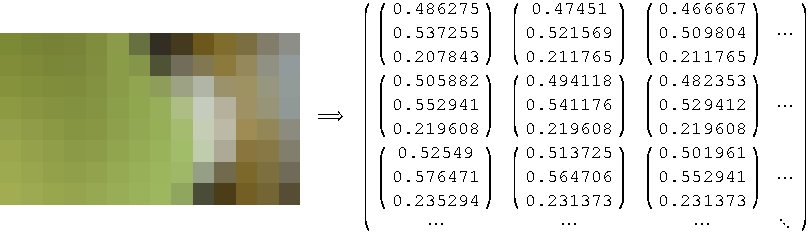
\includegraphics[width=150mm]{image/pic-data.pdf}
\caption{图像的数据结构}\label{fig:pic-data}
\end{figure}

对位图图像中一个像素点亮度的衡量可以有两种方法:一是直接用该像素点的RGB值计算,根据ITU-R BT 601标
准,亮度值$Y = 0.299R + 0.587G + 0.114B$\cite{yuvtorgb}
;二是先把彩色位图转化为灰度位图,由该像素点的的灰度级决定
该点的亮度。对图像中激光斑点的位置进行提取,实际就是确定图像中最亮光斑中心点的位置。由于激光斑点
是一个光斑,而不是一个单一的像素点,图像中最亮像素点的位置也不一定处在光斑的中心,所以对激光斑点
位置的提取需要做进一步探讨。

\section{激光斑点位置提取算法}
\subsection{擂台算法}
如果没有其它杂光干扰,图像中最亮像素点的位置一定在激光光斑的内部,即使不在中心。所以第一步应该确定
最亮像素点的位置,这是比较简单的,可以使用擂台算法。先设一个变量用于存储亮度值,将其初始化为一个较
小的数值,比如零,将这个变量从图像的左上角开始依次与图像的每一个像素的亮度比较,就像打擂台赛,每一
次比较把较大的像素亮度值赋给预设变量,记录下较亮像素点的位置,在扫描完全图后最后留下的像素点的位置
即是该图像中最亮像素点的位置。\textit{Mathematica}程序代码如下。

\begin{verbatim}
briPoint[imgdata_, dim_:{240,320}] := Module[{
    L, (*总行数*)  l, (*总列数*)
    tmp, max=0, (*亮度值*)   x, y (*几何坐标*)
    },
    {L,l} = dim;
    Do[
        tmp = 0.299 * imgdata[[i, j, 1]] + 0.587 * imgdata[[i, j, 2]] 
              + 0.114 * imgdata[[i, j, 3]];
        If[tmp > max,
            max = tmp; x = j; y = L - i + 1;
        ],
        {i,1,L}, {j,1,l}
    ];
    {x, y}
]
\end{verbatim}

程序说明。自定义函数\verb|briPoint[imgdata_,dim_]|用于提取图像中最亮像素点的位置,输入参数
\verb|imgdata|为图像像素值数组,是一个三重嵌套列表,\verb|dim|为该数组的行列维数,是一个列表。
图像数据数组的引索是从图像的左上角开始的,而一个点的几何坐标一般是以图像的左下角为原点的,
程序中对这种情况作了转化。输出值为以图像左下角为坐标原点,以一个像素格点为单位的图像中最亮
像素点的几何坐标。

然而,最亮像素点的位置不一定是在激光光斑的中心,它在光斑内部的位置是不确定的,具有随机性。
实验表明即使激光斑点的位置没有移动,在不同的时间拍摄的图像,计算出的最亮像素点的位置都是
不同的,这与外界光照环境的变化有关。虽然这样基本确定了激光斑点的位置,但其准确度是不可靠的。
为了获得一个稳定的准确的激光光斑的位置坐标,可以采用一种统计的方法,即把光斑范围内所有像素
点的坐标取出,然后对横纵坐标做算术平均,这样可以获得光斑中心的位置,减少外界环境扰动的影响。
算法为在获得图像最亮像素点的亮度值之后不是立刻返回该最亮点的坐标,而是再扫描一遍全图,获取
亮度值低于最亮像素点亮度值一个小量的所有像素点的位置坐标,然后取这些位置坐标平均值。
\textit{Mathematica}程序代码如下。

\begin{verbatim}
briCenterPoint[imgdata_, dim_:{240,320}, di_:0.1] := Module[{
    L, (*总行数*)  l, (*总列数*)
    tmp, max=0, (*亮度值*)   x, y (*几何坐标*)
    points = { } (*光斑像素点坐标集合*)
    },
    {L,l} = dim;
    Do[
        tmp = 0.299 * imgdata[[i, j, 1]] + 0.587 * imgdata[[i, j, 2]] 
              + 0.114 * imgdata[[i, j, 3]];
        If[tmp > max, max = tmp;],
        {i,1,L}, {j,1,l}
    ];
    Do[
        tmp = 0.299 * imgdata[[i, j, 1]] + 0.587 * imgdata[[i, j, 2]] 
              + 0.114 * imgdata[[i, j, 3]];
        (* di 为像素亮度值减去的小量 *)
        If[max-di <= tmp <=max, AppendTo[points, {j, L - i + 1}],
        {i,1,L}, {j,1,l}
    ];
    {x, y} = N@Mean[points];
    {x, y}
]
\end{verbatim}

图\;\ref{fig:postion}为两个程序的运行结果对比图,很明显第二个程序取得的坐标更接近光斑的中心。

\begin{figure}[htbp]
\centering
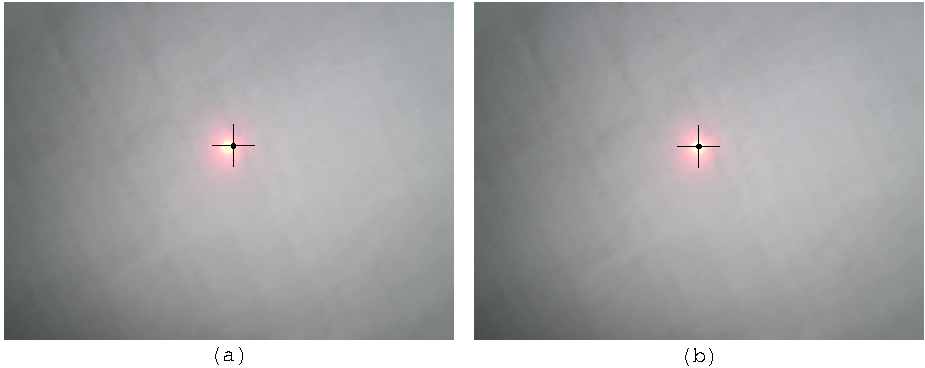
\includegraphics[width=135mm]{image/postion.pdf}
\caption{激光斑点定位效果图\\ (a)为第一个程序的运行结果,(b)为第二个程序的运行结果}\label{fig:postion}
\end{figure}

\subsection{亮中心扩展算法}
上面提到的第二个程序确实提高了激光斑点位置提取的精确度和稳定性,但付出的代价是运算量整整增加了一倍,
因为全图扫描了两遍。自定义函数\verb|briCenterPoint[ ]|的第二个循环,其目的就是获得
激光光斑所在区域所有像素点的坐标。其实为了达到这个目的不一定要再扫描一遍全图。仔细分析,激光斑点所在
区域的所有像素点都是互相连通的,它们聚合成一个亮斑,且整个图像的最亮像素点必然在其中。第二个程序
的第二个步骤是可以再做进一步优化的。可以设计这样一个算法,给定一个阈值作为激光光斑的边界,从最亮像素
点开始,向四周扩展探测,直到扩展完整个光斑区域,这样也能获得激光光斑所在区域所有像素点的坐标。因为是
局域扫描,这种方法可以大大减少计算量。本文称这种算法为亮中心扩展算法,其基本思想是:先检测最亮像素点
上下左右四个像素点哪些满足亮度条件(亮度值是否在光斑亮度值范围内),然后再以这些满足条件的像素点为中
心向外部扩展,即再检测这些像素点的上下左右满足亮度条件的临近点,只选取那些未被检测到的点,以此类推,
直到检测完光斑所在区域所有满足亮度条件的像素点,最后把这些像素点的坐标取平均。具体算法见
流程图\;\ref{fig:briPointExpand-alg}。

\begin{figure}[htbp]
\centering
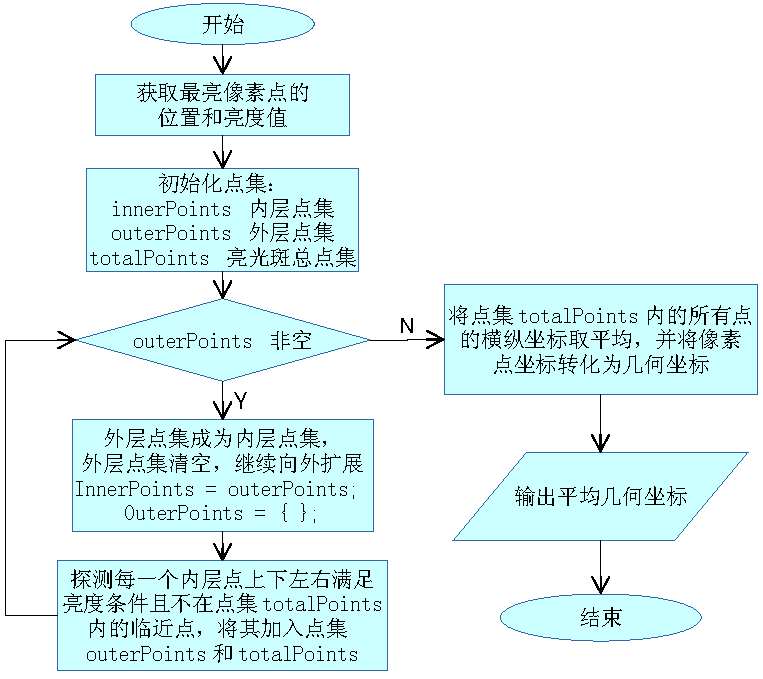
\includegraphics[width=140mm]{image/briPointExpand-alg.pdf}
\caption{亮中心扩展算法流程图}\label{fig:briPointExpand-alg}
\end{figure}

下面是对应的\textit{Mathematica}程序代码,程序中对相关的局部变量和程序段做了详细的注释。

\begin{verbatim}
briPointExpand[imgdata_, maxR_, dim_:{240,320}, di_:0.1] := Module[{
    L, l, (*总行列数*)
    tmp, max = 0, (*亮度值*)
    center, tmpcen, point, (*像素点坐标*)
    totalPoints = { }, innerPoints = { }, outerPoints={ }, (*点集*)
    m, n, x, y (*像素点坐标和几何坐标分量*)
    },
    {L, l} = dim;
    (*先用擂台算法找出最亮像素点的位置和亮度值*)
    Do[ 
        tmp = 0.299 * imgdata[[i,j,1]] + 0.587 * imgdata[[i,j,2]]
              +0.114 * imgdata[[i,j,3]];
        If[tmp > max,
            max = tmp; center = {i, j};
        ],
        {i, 1, L}, {j, 1, l}
    ];
    outerPoints = totalPoints = {center}; (*初始化点集*)
    While[Length[outerPoints] > 0,
        innerPoints = outerPoints;
        outerPoints = { };
        Do[
            tmpcen = innerPoints[[i]];
            (*限制探测范围,探测半径限制在maxR内,且引索不能超过图像边界*)
            If[(Norm[tmpcen - center] < maxR) 
                && (2 < tmpcen[[1]] < L - 1) 
                && (2 < tmpcen[[2]] < l - 1),
                (*探测内层点上下左右像素点是否满足亮度条件*)
                Do[
                    {m, n} = point;
                    tmp = 0.229 * imgdata[[m, n, 1]] 
                          + 0.587 * imgdata[[m, n, 2]]
                          + 0.114 * imgdata[[m, n, 3]];
                    If[(max - di <= tmp <= max) 
                        && (!MemberQ[totalPoints, point]),
                        AppendTo[outerPoints, point]; 
                        AppendTo[totalPoints, point];
                    ],
                    {point, {
                        {tmpcen[[1]], tmpcen[[2]] - 1}, (*左*)
                        {tmpcen[[1]], tmpcen[[2]] + 1}, (*右*)
                        {tmpcen[[1]] - 1, tmpcen[[2]]}, (*上*)
                        {tmpcen[[1]] + 1, tmpcen[[2]]}  (*下*)
                    } }
                ] (* Do *)
            ], (* If *)
            {i, 1, Length[innerPoints]}
        ] (* Do *)
    ]; (* While *)
    {m, n} = N@Mean[totalPoints];
    {x, y} = {n, L - m + 1}; (*把像素点坐标转化为几何坐标*)
    {x, y}
]
\end{verbatim}

由于算法本身有一定的复杂度,自定义函数\verb|briPointExpand[ ]|的代码比较长,但该算法的优化带来的
性能的提升是非常可观的。三个程序的运行情况对比见表\;\ref{tab:result}。

\begin{table}[htbp]
\centering
\caption{三个程序的运行情况对比表}\label{tab:result}
\begin{tabular}{|c|c|c|c|}\hline
函数名   & \verb|briPoint[ ]| & \verb|briCenterPoint[ ]|  & \verb|briPointExpand[ ]| \\\hline
运行结果 & \verb|{163, 138}|  & \verb|{159.558, 137.505}| & \verb|{159.558, 137.505}|\\\hline
运行时间 & 0.406s             & 0.875s                    & 0.422s   \\\hline
\end{tabular}
\end{table}

可见,函数\verb|briCenterPoint[ ]|虽然的到了好的结果,但运行时间是函数\verb|briPoint[ ]|的二倍多,
而函数\verb|briPointExpand[ ]|的运行结果与函数\verb|briCenterPoint[ ]|的完全相同,其运行时间却只
比函数\verb|briPoint[ ]|的多了一点点。

\subsection{多斑点定位}
亮中心扩展算法可以带来另一个好处,就是可以实现多斑点定位。有些实验项目需要同时确定一张图片上两个或
多个激光斑点的位置,这就需要多斑点定位。

函数\verb|briCenterPoint[ ]|的第二步是获得最亮像素点所在的
光斑的所有像素点,其方法是扫描全图,若图像中有多个光斑,一般情况下这些光斑的亮度也比较接近,扫描全
图就不可避免地把其它光斑的像素点采集到,所以函数\verb|briCenterPoint[ ]|对多斑点定位是完全不适用
的。而函数\verb|briPointExpand[]|是可以的,因为函数\verb|briPointExpand[]| 的第二步所用的方法是局部
探测,不同的光斑之间是有界限的,这种方法是不会探测到其它光斑的。

利用亮中心扩展算法进行多斑点定位的方法是:先扫描全图,找到最亮像素点的位置和亮度值,再用亮中心扩展
算法扩展探测该最亮像素点所在光斑的所有像素点,并记录下这些像素点的坐标;然后把这些像素点``遮住'',
开始搜索第二个光斑的位置,方法与找第一个光斑的位置完全相同,只不过避开先前探测到的光斑的像素点;扫
描第三、四个光斑的位置,方法以此类推。具体的程序代码,由于与上面列的多有重复,就不放在正文中了,可
参见附录一。

附录一中共列了三个函数:\verb|briPointHole[ ]|、\verb|pointsDetect[ ]|和\verb|multiSpots[ ]|。
第一个函数\verb|briPointHole[ ]|是对函数\verb|briPoint[ ]|的修改,增加了参数\verb|hole|,它是图像
中被``遮住''的像素点的坐标,返回值为被``遮住''某些光斑后图像中最亮像素点的位置。第二个函数
\verb|pointsDetect[ ]|是对函数\verb|briPointExpand[ ]|的修改,删去了函数\verb|briPointExpand[ ]|%
中搜索最亮像素点位置的部分,保留了亮中心扩展部分,其返回值除了算出的光斑中心几何坐标,还有光斑区域内
所有像素点的几何坐标,这是应该``遮住''的部分。两个函数\verb|briPointHole[ ]|和\verb|pointsDetect[ ]|
配合使用,又构建了另一个函数\verb|multiSpots[ ]|,用于自动搜索图像中多个光斑点的位置。其输入参数之
一\;\verb|n| 是想要搜索的光斑的个数,返回值为图像中指定个数的光斑点的中心坐标。

\section[Mathematica 中的代码编译]{\textit{Mathematica} 中的代码编译}
有些设备对数据采集和分析程序的实时性要求较高,它不仅要实现快速准确的地对激光斑点的位置进行定位,
计算出激光斑点的位移量,甚至要求对所测量的微小量进行实时监控,这就对程序的运行速度提出了很高的要求。
\textit{Mathematica}提供了函数\verb|Compile[ ]|可以对某些程序代码实施编译,第8版的
\textit{Mathematica}还可以调用外部C编译器,把程序编译到机器代码,这可以使程序的运行速度大大提升。

\textit{Mathematica}的变量的类型是动态的,可以在程序运行过程中随时改变,一个变量的数据类型,在程序
运行过程中由\textit{Mathematica}自动检查,这方便了程序的编写,却增加了计算量,而且这只是一方面的
原因。激光斑点位置提取程序所处理的数据对象就是一个三重嵌套的列表(三重数组),处理的都是数据,而没
有任何符号运算,所以是可以编译的。编译就是事先指定所有局部变量的数据类型,尽量使用简单的数学函数,
把\textit{Mathematica}程序代码编译到\textit{Mathematica}虚拟机(MVM)上运行的字节码,这类似于Java。
编译前\textit{Mathemaitca}对局部变量数据类型的判断是依据其初始值的,对输入参数的数据类型的判断要在
\verb|Compile[ ]|函数中明确指定。具体内容可参考\textit{Mathemtica}的官方参考资料中心。

本文提供了自定义函数\verb|briPointExpand[ ]|的编译版本\verb|briPointExpandC[ ]|,见附录二。编译版本
函数\verb|briPointExpandC[ ]|对每一个局部变量进行了初始化,且注意了程序运行过程中一个变量的数据类型
不会改变,把\textit{Mathematica}中内置的两个函数\verb|Norm[ ]|(取向量的模)和\verb|Mean[ ]|(取数
据的平均值)替换为结构化程序代码段,以实现编译。经测试,函数\verb|briPointExpandC[ ]|的运行结果与
函数\verb|briPointExpand[ ]|的完全相同,但把运行时间从0.422秒缩短到0.015秒,速度提升了28倍!

\section{定点干涉条纹扫过数量的自动计数}
利用激光进行微小位移测量的另一种方法是激光干涉法,其中涉及到对扫过定点干涉条纹的自动计数。这里相关
的程序算法和上面的是完全不同的。本文将对移动着的条纹自动计数方法和有关的问题做一般性的论述。

编制定点干涉条纹扫过数量的自动计数程序,要解决两个问题:一是动态,即实时跟踪在干涉条纹移动方向上有
关像素点集的亮度值;二是条纹特征检测,即根据动态变化的条纹纵切线像素点集亮度值,如何判断条纹是否移动了以及如何计数。

第一个问题是好解决的,可以利用这种形式\verb|Dynamic[process[CurrentImage[]]]|,
对CCD图像中指定位置的像素点集的亮度值进行跟踪。其中\verb|process[ ]|是像素点集提取函数,根据函数
\verb|Dynamic[ ]|的功能特点,像素点集提取函数\verb|process[ ]|的输出结果必须在屏幕上可见,这样才能
动态地刷新所需位置像素点集的亮度值,实现跟踪。处理程序\verb|process[ ]|提取的像素点亮度值集合可以
通过一个全局变量传递给其他程序,以对条纹特征进行识别。下面给出一个该处理程序的实例。

\begin{verbatim}
fringesDataGet[img_, centerG_, sd_, d_, dim_:{240, 320},size_:400] := 
  Module[{
    imgdata, (*图像数据*)
    x, y, (*扫描中心几何坐标分量*)   L, l, (*图像大小*)
    tmp, (*像素点亮度值*)  tmpdata, (*暂存条纹亮度值数据*)
    (* fringesData 为全局变量,用于传递条纹亮度值数据*)
    },
    {x, y} = centerG;  {L, l} = dim;
    tmpdata = { };
    imgdata = ImageData[img];
    (*扫描指定位置的条纹亮度值数据*)
    Do[
        tmp = 0.229 * imgdata[[i, x, 1]] + 0.587 * imgdata[[i,x,2]] 
              + 0.114 * imgdata[[i, x, 3]];
        PrependTo[tmpdata, tmp],
        {i, L - y + 1 - sd, L - y + 1 + sd}
    ];
    fringesData = tmpdata; (*更新条纹亮度值数据, fringesData 为全局变量*)
    (* 可视化结果 *)
    Framed@Row[{
        Show[ (*绘制扫描到的条纹亮度值数据曲线*)
            ListLinePlot[fringesData,
                Frame -> True, PlotStyle -> Darker[Green], 
                PlotRange -> {-0.1, 1.1}, AspectRatio -> (3 / 4),
                ImageSize -> size
            ],
            Graphics[{
                {Blue, Dashed, Line[{{1, 0}, {1, 1}}], 
                               Line[{{2 * sd + 1, 0}, {2 * sd + 1, 1}}] },
                {Red, Line[{{sd + 1, 0},{sd + 1, 1}}], 
                      Line[{{sd + 1 - d, 0}, {sd + 1 - d, 1}}],
                      Line[{{sd + 1 + d, 0}, {sd + 1 + d, 1}}] }
            } ]
        ],
        Show[ (*在图像中标明数据扫描的位置和范围*)
            img,
            Graphics[{
                {Darker[Green], Line[{{x, y - sd}, {x, y + sd}}] },
                {Red, Line[{{x - 50, y}, {x + 50, y}}],
                      Line[{{x - 50, y - d}, {x + 50, y - d}}],
                      Line[{{x - 50, y + d}, {x + 50, y + d}}] },
                {Blue, Dashed, Line[{{x - 50, y - sd}, {x + 50, y - sd}}],
                               Line[{{x - 50, y + sd}, {x + 50, y + sd}}] }
            }], 
            ImageSize -> size
        ] 
        }, Spacer[20] ]
]
\end{verbatim}

函数\verb|fringesDataGet[img_, centerG_, sd_, d_, dim_, size_]|的参数\verb|img|为直\\
接从CCD摄像头获取的图像(\verb|CurrentImage[ ]|),\verb|centerG|为目的定点
的几何坐标,\verb|sd|为数据扫描的宽度,扫描到的数据传递给全局变量\verb|fringesData|,以供条纹计数
程序使用,\verb|d|为条纹计数程序要处理的样本数据的宽度。函数\verb|fringesDataGet[ ]|的输出为实时
动态的可视化图像,这要结合动态函数\verb|Dynamic[ ]|的使用。该函数的输出与运行效果见
图\;\ref{fig:fringes-count} 。

\begin{figure}[htbp]
\centering
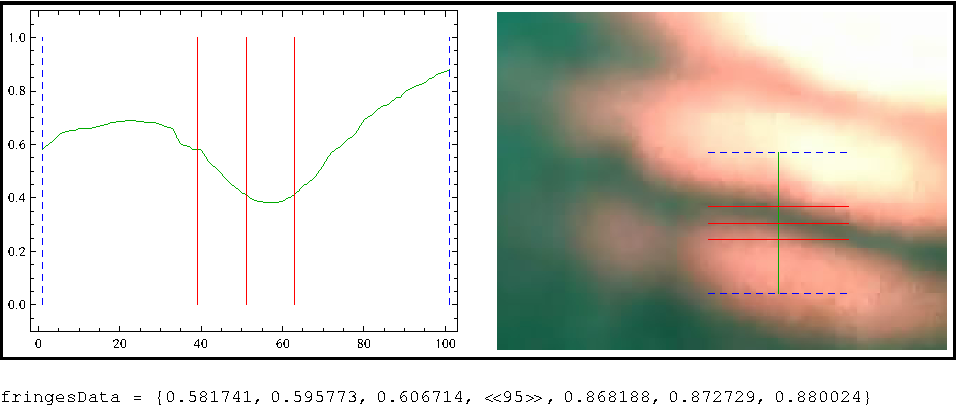
\includegraphics[width=150mm]{image/fringes-count.pdf}
\caption{函数fringesDataGet[\;]的运行效果图}\label{fig:fringes-count}
\end{figure}

难度在于第二个问题,即根据函数\verb|fringesDataGet[ ]|获得的干涉条纹亮度数据,如何即时分析条纹的
特征,判断条纹是否移动、移动的方向和移动的个数。由于各种外界环境的干扰和随机因素,实际得到的条纹
亮度曲线并不是非常光滑的。得到的条纹亮度曲线整体上看是波浪形的,而仔细观察曲线,却存在许多细小的
毛刺,这也给相关的数据处理带来困难。

\begin{figure}[htbp]
\centering
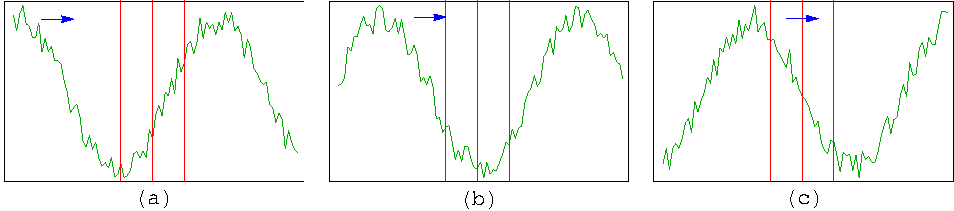
\includegraphics[width=150mm]{image/line-fringes-2.pdf}
\caption{干涉条纹特征检测}\label{fig:line-fringes-2}
\end{figure}

本文采用一种统计的方法。如图\;\ref{fig:line-fringes-2} ,在所获得的条纹亮度数据中设定两条距离不大
于半个条纹宽度的边界线,仔细观察,随着条纹的移动,这两条边界线之间的条纹亮度数据的统计特征是不同
的,可以根据这个统计特征判断条纹的移动状态。图中的箭头表明条纹移动的方向,图中有三条红线,从左到
右分别定义为左线、中线和右线。在图\;\ref{fig:line-fringes-2}a 中,左右两线之间的像素点亮度值大多
数都大于左线所在处的像素点的亮度值,小于右线所在处的像素点的亮度值;干涉条纹向右移动一点后,到达
如图\;\ref{fig:line-fringes-2}b 所示的情况,这时左右两线之间的像素点亮度值基本上都小于左线所在位
置的像素点亮度值,也基本上都小于右线所在处的像素点亮度值;干涉条纹继续移动,到达如
图\;\ref{fig:line-fringes-2}c 所示的情况,这时与图\;\ref{fig:line-fringes-2}a 的情况正好相反,
在左右两线之间的像素点亮度值基本上都小于左线所在位置的像素点亮度值,基本上都大于右线所在位置的像素
点的亮度值。根据这些特征的不同,就可以判断条纹的位置变化了。首先设计三个选判器(判断条件),分别
能够判断在观测点处条纹所处的上述三种情况。由于数据是实时变化的,而条纹移动数量的计数却是间断性的,所
以还应该设置一个计数开关,控制计数的进程。这个计数开关可以这样设置,当条纹移动到如
图\;\ref{fig:line-fringes-2}b 所示的情况时,打开计数开关,随着条纹的移动,若检测到条纹处在如
图\;\ref{fig:line-fringes-2}c 所示的情况,则计数器加\;1 ,并立刻把计数开关关掉,以避免重复计数。
如果此时条纹移动的方向改变,改为向左移动,当条纹经过如图\;\ref{fig:line-fringes-2}b 所示的情况时,
计数开关又打开,随着条纹的移动,条纹会经过如图\;\ref{fig:line-fringes-2}a 所示的情况,这时使条纹
计数器减\;1 。这种方法所测的是干涉条纹单方向移动数量。下面给出具体的\textit{Mathematica}程序代码。

\begin{verbatim}
fringesCount[fringesData_, sd_, d_, imin_:0.2, imax_:0.8, igap_:0.05]:=
  Module[{
    sampleData = { }, (*样本数据*)
    first, last, mean, len,
    boolFirst = { }, boolLast = { },
    boolMeanFirst, boolMeanLast, (*布尔值平均*)
    (*countFlag 为全局变量,是计数开关,其初始值为 True *)
    (*counter 为全局变量,是单方向条纹计数器,其初始值应设置为 0 *)
    (*total 为全局变量,是总共经过的条纹数,不论方向,初始值也为 0 *)
    (*该函数运行前要对这三个全局变量初始化,否则会运行出错*)
    },
    (*提取样本数据*)
    Do[
        AppendTo[sampleData, fringesData[[i]]], 
        {i,sd + 1 - d, sd + 1 + d}
    ];
    len = Length[sampleData];
    (*特征统计量的计算*)
    first = First[sampleData];
    last = Last[sampleData]; 
    mean = Mean[sampleData];
    Do[
        AppendTo[boolFirst, Boole[sampleData[[i]] > first]];
        AppendTo[boolLast, Boole[sampleData[[i]] > last]],
        {i, 2, len - 1}
    ];
    boolMeanFirst = Total[boolFirst] / (len - 2);
    boolMeanLast = Total[boolLast] / (len - 2);
    (*条纹特征识别*)
    If[countFlag, #]&@Which[
        (*第一种情况*)
        (boolMeanFirst <= imin) && (boolMeanLast >= imax)
        && (first - mean >= igap) && (mean - last >= igap), 
        counter++; total++; countFlag = False,
        (*第三种情况*)
        (boolMeanFirst >= imax) && (boolMeanLast <= imin)
        && (mean - first >= igap) && (last - mean >= igap),
        counter--; total++; countFlag = False
    ];
    (*第二种情况*)
    If[(!countFlag)&&(boolMeanFirst <= imin) && (boolMeanLast < = imin)
       && (first - mean >= igap) && (last - mean >= igap),
        countFlag = True (*打开计数开关*)
    ]
   {counter, total}
]
\end{verbatim}

函数\verb|fringesCount[ ]|也要与函数\verb|Dynamic[ ]|配合使用,以实现对全局变量\\
\verb|fringesData|
的动态跟踪。函数\verb|fringesCount[ ]|的三个输入参数\verb|imin|、\verb|imax|和\verb|igap|都是统计
量。这三个统计量的数值与干涉条纹图像的质量有关。干涉条纹越清晰,外界干扰越小,就要把参数\verb|imin|
设置的越小,把参数\verb|imax|设置的越大,参数\verb|igap|也要适当的增大,这样计数就越准确。反之,若
干涉条纹比较模糊,不容易分辨,应该把参数\verb|imin|增大,把参数\verb|imax|和\verb|igap|减小,但这样
可能会出现误计数的情况。要保证\verb|imax|
比\verb|imin|大,否则条纹移动的记录方向会反向,输出的\verb|counter|值会是负的。一般情况,要保证参数
\verb|imin|和\verb|imax|的和为\;1 。

函数\verb|fringesDataGet[ ]|进行实时跟踪获取条纹亮度值数据,并把数据传递给全局变量
\verb|fringesData|,函数\verb|fringesCount[ ]|则随时检测全局变量\verb|fringesData|的数据,识别条纹
的特征,对条纹的扫过指定点的移动数量进行单方向计数。这两个函数配合,从图\;\ref{fig:fringes-count} 
看,其计数方向是向上,在实际计数时注意把CCD摄像头调整到适当方向。

还有一个问题需要注意。若干涉条纹移动到如图\;\ref{fig:line-fringes-2}b 所示的情况,计数开关打开,
但这时正好没有再继续向右移动,而是立刻反向了,条纹移动到如图\;\ref{fig:line-fringes-2}a 的情况,
而不是图\;\ref{fig:line-fringes-2}c ,这时就有可能误计数,使条纹移动计数器减\;1 。不过这种情况出
现的概率是很小的,在实际测量中也要注意一下这种情况,尽力避免干涉条纹反向移动。

\section{程序模块设计}
前面详细地探讨了利用激光进行微小位移测量所涉及到的最核心的图像处理算法:CCD图像中激光光斑位置的
自动提取算法和干涉条纹移动数量的自动计数方法,并给出了核心函数的程序源代码。下面将利用这些函数开始
构建实际可用的整个软件系统所必须的程序组件。

实际使用的整个软件系统的设计方案是模块化设计。每个模块都各有自己的分工,负责不同的工作,模块之间
通过全局变量通信。

对于不需要动态跟踪的比较简单
的系统,比如只根据两张图片单次计算激光斑点的移动数量,并一次换算出所测量微小位移量的数值,只需要设置
两个模块即可,一个是拍照模块,另一个是计算模块。拍照模块只负责拍摄两张含有激光斑点的图片,计算模块
只要做三项工作,先从两张图片中提取出激光斑点的位置,然后把两个位置坐标做差,求出这两点以一个像素为
单位的图像距离,再根据事先测量的比例系数换算成激光光斑的实际移动距离,最后算出所测量微小量的数值并
输出。

而对于需要动态跟踪、实时监控的系统,其模块组成要复杂得多。由于要求测量过程是即时的、动态的、自动的,
这就要利用\textit{Mathematica}从2007年第\;6 版引进的革命性的动态功能\verb|Dynamic[ ]|。每个模块
都由函数\verb|Dynamic[ ]|包装,以实现动态模块,\textit{Mathematica}即时地更新从CCD摄像头获取的图像,
并利用自定义函数进行动态地处理,把处理的结果赋值给全局变量,供其他模块使用。其他模块也设置为动态
模块,当其引用的全局变量更新时,该模块也自动重新计算。所以从CCD获取的图像不仅是整个软件系统的数据
源,也是动态触发源。

利用光杠杆法测量微小位移量所需的动态软件监控系统,需要如下几个程序模块。(1)图像获取与斑点位置提取
模块,用于即时地从CCD摄像头采集图像,并即时地提取出激光斑点所在的位置,把位置坐标传递给全局变量,
这个位置坐标是随着光斑的移动而动态变化、实时更新的。(2)比例系数测量模块,用于测量图像距离与实际距
离的换算比例。(3)数据转化与动态图表模块,根据换算比例把图像距离转换成实际位移,并根据相关的物理原
理即时算出所测量的微小位移量,然后用图表动态的表示计算结果,包括方向和大小,如果遇到异常数据及时做
出预警。(4)数据在线储存模块,用于在线地把所测量到的数据以一定的格式储存到计算机硬盘,以供测量完成
后做数据分析。

\subsection{图像获取与激光斑点位置提取模块}
软件系统主程序的构建主要利用\textit{Mathematica}的内置函数\verb|Manipulate[ ]|。内置函数
\verb|Manipulate[ ]|的基本应用形式是
\verb|Manipulate[被操纵的对象, {控件或模块1}, {控件或模块2},...]|,
其输出为一个窗体对象,该窗体对象的逻辑结构见图\;\ref{fig:manipulate} 。

\begin{figure}[htbp]
\centering
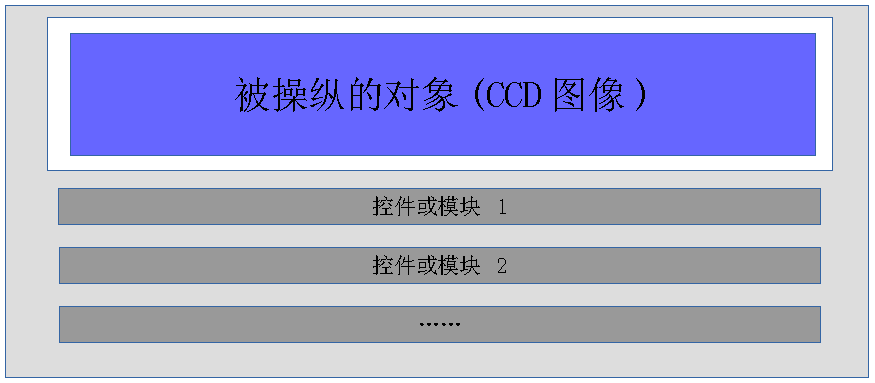
\includegraphics[width=130mm]{image/manipulate.pdf}
\caption{函数Manipulate[ ] 输出的窗体对象的逻辑结构}\label{fig:manipulate}
\end{figure}

图像获取与激光斑点位置提取模块位于``被操纵的对象''部分,是整个软件系统的数据源和动态触发源。
只要应用前面定义的激光斑点位置提取函数为结构\verb|Dynamic[process[CurrentImage[],...]]|中的处理程
序\verb|process[ ]|定义一个实例,其计算过程中要把即时激光斑点的位置传递给全局变量,其输出为激光斑
点的初始位置和即时位置的动态可视化图像。在定义处理程序\verb|process[ ]|的实例时,为了提高程序的运
行速度,可应用激光斑点位置提取函数的编译版本。另外为了实现对该处理程序工作状态的有效控制,应在其输
入参数中加一些控制开关。

与程序模块有关的程序代码就不放在正文中了,图像获取与激光斑点位置提取模块的处理程序实例见附录三提供
的函数\verb|processCCD[ ]|。图\;\ref{fig:processCCD-result} 为函数\verb|processCCD[ ]|的运行测试结
果。运行结果中两根红虚线指示的是激光斑点
初始位置,蓝实线指示的是激光斑点的当前位置,其具体数值由图下的\verb|P0|和\verb|P1|标明。

函数\verb|processCCD[]|的应用方法应为如下的方式,其它模块可调用函数\verb|processCCD[]| 动态刷新的
全局变量\verb|currentDistance|,即当前激光斑点位移的图像像素距离。
\begin{verbatim}
Manipulate[
    Dynamic[processCCD[CurrentImage[], <初始位置>, <监控开关>, ...]],
    Item[ ... ], (*模块 1*)
    Item[ ... ], (*模块 2*)  ...
]
\end{verbatim}

\begin{figure}[htbp]
\centering
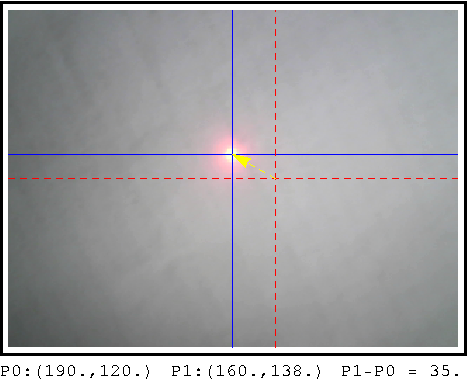
\includegraphics[width=100mm]{image/processCCD-result.pdf}
\caption{函数processCCD[ ]的运行测试结果}\label{fig:processCCD-result}
\end{figure}

\subsection{比例系数测量模块}

从图像的像素距离换算成实际距离还需要一个换算比例系数。在微小量测量的过程中,CCD摄像头和光屏之间的
距离一般是不改变的,这个换算比例系数也是不变的。程序中应该内置一个比例系数测量模块。

\begin{figure}[htbp]
\centering
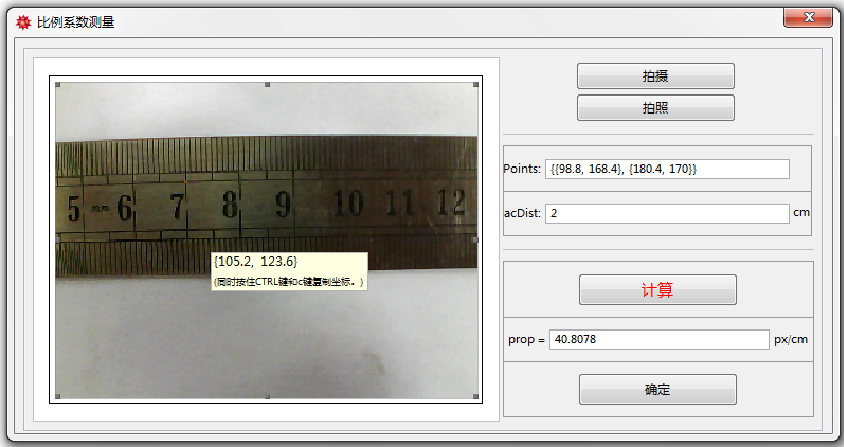
\includegraphics[width=130mm]{image/proportion.pdf}
\caption{函数getProportion[]的运行结果,比例系数测量程序界面}\label{fig:proportion}
\end{figure}

该模块的设计思路很简单。预先在光屏上选定两个已知距离的点,然后启动摄像头拍照,利用\textit{Mathematica}
手动选取这两个点的坐标,并计算出这两点的图像像素距离和实际距离的比,这个比就是所要测量的比例系数,最后
通过全局变量把测得的比例系数传递给其他程序模块使用。附录三中的函数\verb|getProportion[]|给出了该模块
的示例程序代码 。函数\verb|getProportion[]|通过全局变量\verb|proportion|传递所测得的比例系数。
图\;\ref{fig:proportion} 为该模块示例程序的运行界面。

\subsection{数据转化与动态图表模块}
当知道了激光斑点位移的图像像素距离和比例系数,就能计算出光斑的实际移动距离了,这时就可以着手计算所需测量
的微小位移量了。这要结合输入的与仪器相关的其它物理量,比如光程,利用光杠杆放大原理进行计算。由于光斑的
移动距离是随时变化的,该模块要设置成动态模块,定时检查全局变量\verb|currentDistance|,计算所测微位移的大
小,并可视化输出,输出的图表是定时刷新、动态变化的,以实现对所微位移的监控。

这里的数据转换是与具体的实验仪器和研究项目有关的,所以不再详细讨论,只说一下相关的图表怎么构建。这里涉及
到的图表有两种,一种是即时方向指示表盘,另一种是所测微小位移量动态监控曲线图。前者很容易实现,同样是利用
\verb|Dynamic[process[currentPosition, ... ]]|结构,注意\verb|currentPosition|(当前激光
斑点的位置,由函数\verb|processCCD[ ]|动态刷新)是即时变化
的全局变量,由于
\verb|Dynamic[ ]|的作用,这个全局变量每一次更新都会引起该模块的重新计算。只需要设法算出当前光斑位置相对于
初始光斑位置(\verb|originalPosition|)的方向角并用数字仪表盘可视化表示即可。后者也比较容易实现,
只需要注意两点,微小位移量动态监控曲线的数据
量必须固定,数据的刷新最好是定时,而不应该由全局变量\verb|currentDistance|的更
新来触发,因为全局变量
\verb|currentDistance|的更新可能很快,监控曲线图更新太快就没法辨认。定时刷新的方法可以用下面的方式。
\begin{verbatim}
Dynamic[
    Refresh[process[currentDistance, ...], UpdateInterval -> t], 
    TrackedSymbols -> { }
]
\end{verbatim}

代码中\verb|TrackedSymbols->{}|指明不跟踪任何符号,\verb|UpdateInterval->t|指明定时刷新的时间间隔是
\verb|t|秒。

监控曲线图的每一次更新只要做三件事情,先把数据容器最前面最早的一个数据删除
(\verb|Drop[expr, 1]|),在数据容器最后面加入最新的数据(\verb|Append[]|),再用
函数\verb|ListLinePlot[ ]|可视化数据。这里的数据容器应该是全局变量,这不是为了向其它模块传递数据,
而是为了保留历史记录。具体的程序代码比较简单,不再详述。

\subsection{数据在线储存模块}
有些实验项目要求定期地在线储存所测得的数据,以供在测量完成后进行数据分析。储存的数据内容要根据具体的实验项
目确定。一般情况下数据是按时间的顺序储存的,在每一个时间点储存的是一个数据单元,其格式可以按下面的方式。
\begin{verbatim}
<起始时间>; {<时间偏移1>,{<数据单元1>}}; {<时间偏移2>, {<数据单元2>}}; ...
\end{verbatim}

\verb|<起始时间>|是数据记录的起始时间,可以用函数\verb|AbsoluteTime[]|计算,其计算结果为实验地点
所在时区从1990年1月1日到当前时刻为止的总秒数。\verb|<时间偏移n>|为\verb|<数据单元n>|记录时的时间与起始时间的差
值,单位为秒。不同的数据单元以分号\verb|";"|分隔。

对于数据的在线储存,本文不再详述具体的程序代码,只说一下相关的流程和注意事项。
(1)在数据储存开始之前应该定义一个
设置窗口,用于设置数据储存的文件位置、数据储存的起止时间、数据单元记录的时间间隔,并打开写入数据文件流
(\verb|OpenWrite[ ]|),写入\verb|"<起始时间>;"|,做好数据在线储存的准备。
(2)定义数据储存函数,要做两项工作,
一是数据转化和准备,二是向指定的数据文件流写入数据,注意写入的数据为字符串流,应使用函数\verb|WriteString[ ]|,
并且写入的数据要用函数\verb|ToString[ ]|转化成字符串。每写入一个数据单元,不要忘记写入分隔符\verb|";"|。
到达数据储存结束时间或中途终止记录时要关闭打开的数据文件流(\verb|Close[ ]|)。
(3)数据储存模块也要采用定时刷新的方式,其刷新时间间隔就是数据单元记录的时间间隔。另外数据储存模块在程序
界面中一定要有输出,表明数据记录的状态、已记录数据单元的个数,这也是为了实现动态,不在程序窗口中显示的
\verb|Dynamic[ ]|结构是不会自动重新计算的。
(4)在数据分析读取数据时可用这种形式
\verb|ToExpression@Read[str,Record,RecordSeparators->";"]| 读入起始时间或一个数据单元,其中\verb|str|
为打开的读入数据文件流(\verb|OpenRead[ ]|)。当读到文件末尾时函数\verb|Read[ ]|将返回\verb|EndOfFile|。

\subsection{干涉条纹移动数量自动计数模块}
对于干涉条纹移动数量的自动计数,前面已经探讨并定义了两个函数\\
\verb|fringesDataGet[]| 和\verb|fringesCount[ ]|,
函数\verb|fringesDataGet[ ]|用于即时获取指定位置的干涉条纹亮度数据,并把数据传递给全局变量
\verb|fringesData|。函数\verb|fringesCount[ ]| 用于动态监视全局变量\verb|fringesData|,即时分析数据的统计特征,
辨别条纹移动的状态,对条纹的移动数量进行计数,计数结果由全局变量\verb|counter|和\verb|total|传递。
干涉条纹移动数量自动计数模块就是要把这两个函数整合起来,使它们配合工作。该模块要放在函数\verb|Manipulate[ ]|
中``被操纵的对象''部分。具体的构建方式如下。

\begin{verbatim}
Manipulate[
    Column[{
        Dynamic[fringesDataGet[CurrentImage[], ... ]],
        Dynamic[
            If[start,
                fringesCount[fringesData, ... ],
                {counter, total}
            ]
        ]
    }],
    Item[ ... ], 
    Item[ ... ], ... ,
    Initialization :> (counter = total = 0; countFlag = True)
]
\end{verbatim}

其中\verb|start|为计数开始开关,一定要在函数\verb|fringesDataGet[ ]|运行后才能开始计数,否则计数函数
\verb|fringesCount[ ]|会因为全局变量\verb|fringesData|中没有数据而运行出错。

\section{整个应用程序系统的组建}

探讨完各个程序模块的设计,下面开始着手组建整个应用程序系统。把上面的各模块整合起来,与实际的实验项目相
结合,具体说明上述有关算法的实际应用和软件系统的整体组建方法。下面以我们学院在2011年和2012年山东省大
学生物理科技创新大赛中的利用激光进行微位移测量有关的程序项目为例进行说明。

\subsection{固体液体折射率的自动化测量}

激光斜射入透明固体或液体介质会改变传播方向,方向改变的大小与介质的折射率有关,根据这个原理可以测量介质
的折射率。用这种方法测量折射率具体来说是不需要测量微小位移的,但它需要测量激光斑点的位移,因为介质会改
变激光的传播方向,从而引起终端接收光屏上激光斑点的移动,通过这个移动的大小可以推算相关的角度,并由此
算出所测介质的折射率。该测量一般属于单次测量,不需要动态监控,所以相应的程序系统比较简单。只需要手动
拍摄两张照片,一张是激光不经过介质时的光屏图像,另一张是激光经过介质时的光屏图像。再设置一个``计算''
按钮,用于提取这两张照片中的激光斑点的位置,计算两个激光斑点的实际距离,并由此计算并输出所测量的折射
率。相应的程序界面见图\;\ref{fig:zheshelv} 。

\begin{figure}[htbp]
\centering
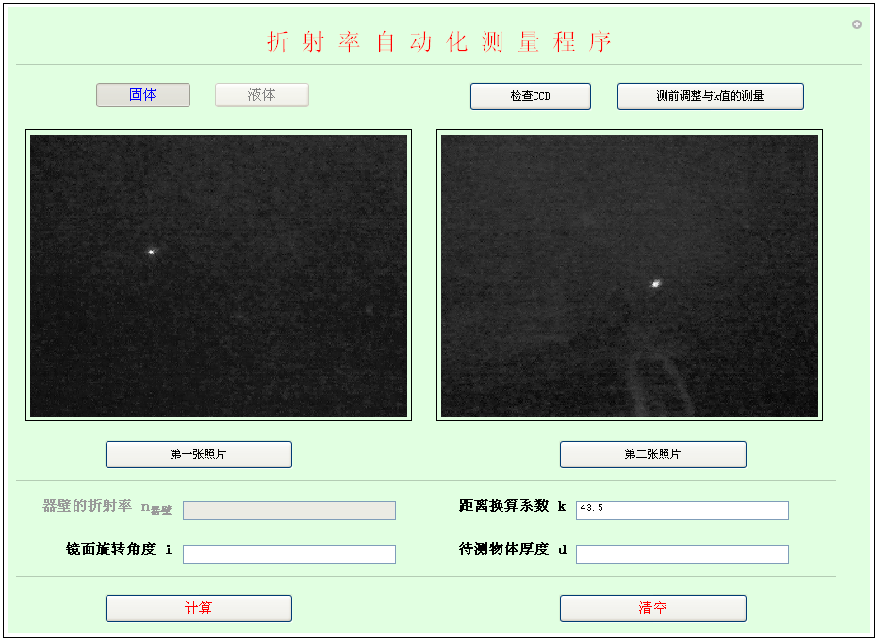
\includegraphics[width=99mm]{image/zheshelv.pdf}
\caption{固体液体折射率测量程序}\label{fig:zheshelv}
\end{figure}

主程序都是在\verb|Manipulate[ ... , Item[ ... ], Item[ ... ], ...]|结构中。程序界面中各种控件,如按钮、
输入框、滑块等的位置安排可以使用函数\verb|Row[ ]|、\verb|Column[ ]| 和\verb|Grid[ ]|。
图\;\ref{fig:zheshelv} 所示的折射率自动化测量程序有两种工作模式,
一种是测量固体,一种是测量液体,在程序的左上角有两个切换按钮。``检查CCD''按钮用于初次启动CCD设备,检测
其是否工作正常。``测前调整与k值的测量''就是比例系数测量模块,同时在该模块的摄像状态下还可以调整仪器设备,
如摄像头的方向、摄像头与光屏的距离等。程序中间是拍照模块,拍照的方法就是直接把
函数\verb|CurrentImage[]|的返回值赋给全局变量,供计算模块使用。计算模块就是下面红色的``计算''按钮,直接
单击就可以立刻根据两张照片和输入的参数计算并输出所测折射率的数值结果。

\subsection{垂直摆地倾斜测量仪}

地面倾斜角的测量对于地质、地震等的研究具有重要意义。地倾斜角一般是非常微小的,所以该项目属于微小角度
测量,所用的测量方法是光杠杆原理。该项目对所需的程序系统有两个要求:一是实时监控,对过大倾斜角做出报警,
这对于地震前兆的预警有作用;二是数据在线储存,这主要是为了测后研究地面倾斜角的变化规律,包括大小和方向。

具体的程序界面见图\;\ref{fig:chuizhibai} ,这是一个典型的需要实时动态监控所测量的微小量和在线数据储存
的程序系统。程序的左上方就是上述的图像获取与激光斑点位置提取模块,当开始拍摄和监控时,该模块即时刷新两
个全局
变量,一个是当前激光斑点的位置坐标\verb|currentPosition|,另一个是当前激光斑点相对于其初始位置的位移
\verb|currentDistance|。初始位置的获取由程序界面右上方的控制面板负责,其中有一个``获取初始照片''按钮,
单击它,就会自动拍摄一张照片作为初始照片,并计算出其中激光斑点的位置,将其传递给全局变量
\verb|originalPosition|,供其它模块使用。注意初始位置这个全局变量一旦获取,在程序的整个运行期间是不变
的,而激光斑点的当前位置和相对位移两个全局变量是即时变化的,这是整个程序的数据源。在程序界面的控制面板
部分内置了一个比例系数测量模块,单击``比例系数测量''按钮即可启动。在程序界面的下方是数据转化与动态图表
模块。该模块分为左右两部分,其中左边是倾斜方向监控表盘,其监控的主要数据对象是全局变量
\verb|currentPosition|,该部分被设计为即时刷新的,因为一般情况下地倾斜方向的变化不会很快,不会影响对表
盘指针的观察;右边部分是地倾斜角大小动态监控曲线图,其监控的数据对象是全局变量\verb|currentDistance|,
曲线图的最右边是最新数据,左边是历史数据,该部分被设计为定时刷新的,即刷新时间是可控的,这是因为全局变
量\verb|currentDistance|是即时变化的,速度很快,若根据它的变化来触发监控曲线的更新,会使监控曲线向左
``流动''得太快而难以辨认。在程序界面右上方控制面板部分中的四个较长的按钮和``数据储存状态''区域是数据在
线存储模块。``数据储存设置''按钮用于设置数据储存的位置、数据储存的计划起止时间和数据元记录的频率,并打
开数据文件流,为数据在线储存做好准备。``数据储存状态''下的文字是动态数据储存函数的输出,数据储存函数可
以根据已设的起止时间自动开始数据记录和停止记录并关闭数据文件流。数据记录的进程也可由控制面板中的相关
按钮控制。有关仪器设备的参数,如光程、倾斜角警戒值等的输入,可以单击控制面板中的``参数设置''按钮,会弹
出数据输入窗口,用于参数的输入,输入的参数会反馈到程序界面中间``已设参数''部分。


\begin{figure}[htbp]
\centering
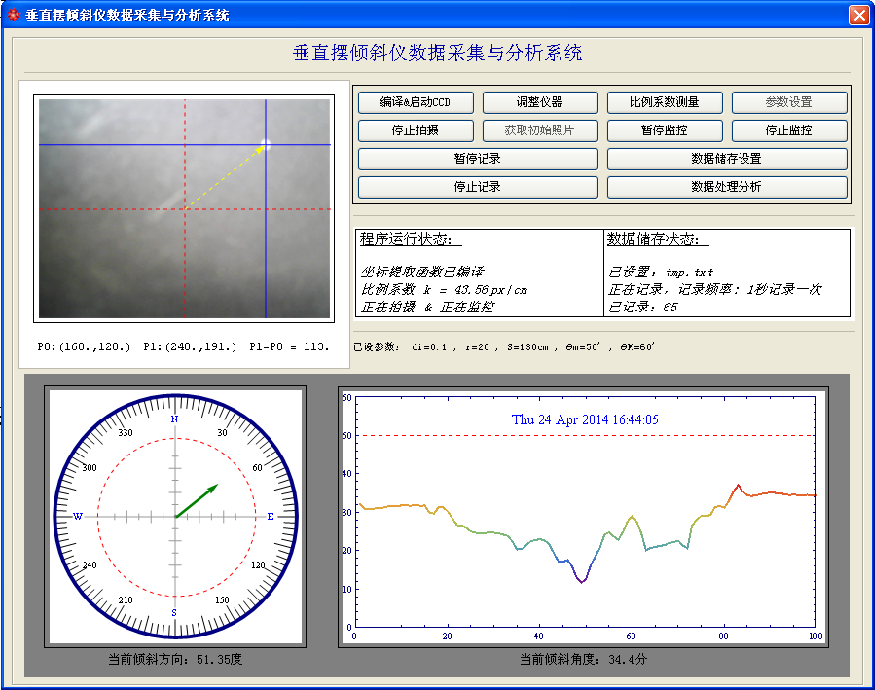
\includegraphics[width=120mm]{image/chuizhibai.pdf}
\caption{垂直摆地倾斜测量仪数据采集与分析系统}\label{fig:chuizhibai}
\end{figure}

\subsection{表面张力系数自动化测量}

\begin{figure}[htbp]
\centering
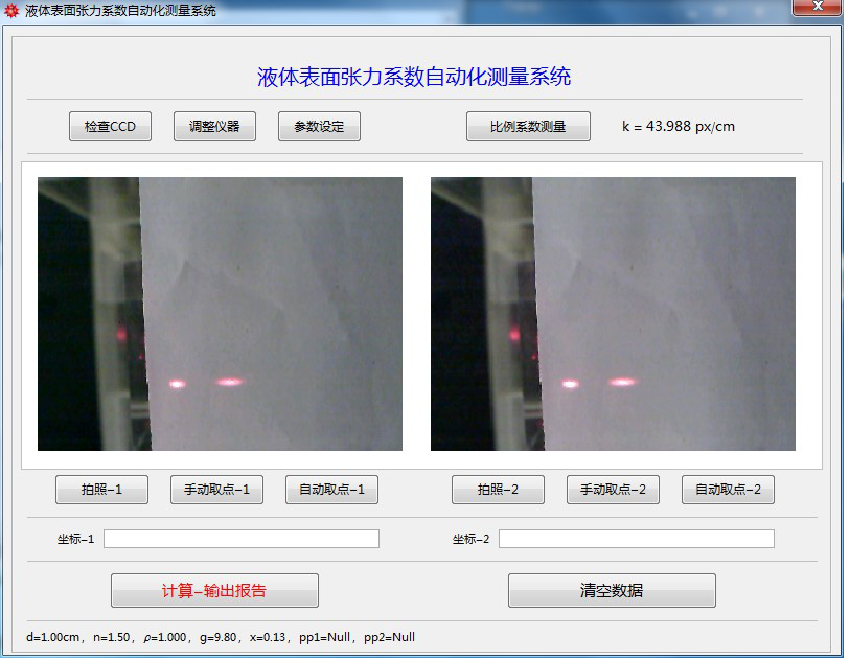
\includegraphics[width=120mm]{image/biaomianzhangli.pdf}
\caption{表面张力系数自动化测量程序}\label{fig:biaomianzhangli}
\end{figure}

该项目提出了一种全新的测量液体表面张力系数的方法,利用两束极细的距离很近的激光竖直向下投射到待测液体平面
与容器壁的交界处,由于侵润和液体表面张力的作用,该处会形成一个曲面,会把两束激光分别向不同的方向反射。根
据这两个不同的反射角就可以推算出待测液体的表面张力系数,这样就把对表面张力系数的测量转化为对这两个反射角
的侧量。该项目与前面折射率的侧量相似,都是对激光光线的有关角度进行测量,而且只是单次测量,不需要动态跟踪。
但与折射率的测量不同的是,在该项目中有两束激光,需要同时测量两个激光斑点的位移,这就涉及到了多斑点定位。

该项目的程序界面见图\;\ref{fig:biaomianzhangli} ,程序中同样设置了两个拍照按钮,需要注意的是,这里拍摄到
的每张照片中都有两个激光斑点。在每个拍照按钮旁边又分别设置两个按钮,一个是手动取点,另一个是自动取点,
意思是可以通过手动和自动两种方法获取图像中两个激光斑点的位置坐标。手动的方法利用的是\textit{Mathematica}
的内置功能,在图像质量很差,图像中有很多干扰的情况下可以手动取点,
要把手动取得的两个激光斑点的位置坐标粘贴到主程序中相应的输入框中。
自动取点就利用到了前面论述的多斑点定位
的方法,前面已给出了具体的算法和程序代码。当拍完照片,单击``自动取点''按钮,就可以进入到自动取点程序,界
面见图\;\ref{fig:twospots-detect} 。程序界面右上方是探测区域控制滑块,用于缩小激光斑点的探测范围,去除全
图其他区域杂光的影响。下面的两个输入框分别用于设定激光斑点亮度阈值和激光斑点最大容许半径。只要把探测区域
和这两个参数设置好,单击``计算''按钮,就可以自动计算出两个激光斑点的位置坐标,再单击``确定''按钮,就可以
把这两个位置坐标赋值到有关的全局变量,自动``输入''到主程序界面中相应的输入框中。在取完两张照片中激光斑点
的位置后,单击``计算-输出报告''按钮,程序就自动根据这四个点的坐标计算两个激光斑点的位移,进而计算出两个
反射角的大小并计算和输出所测液体的表面张力系数。该程序还内置了一个数据储存程序,用于把每次测量的数据储存
到文本文件。

\begin{figure}[htbp]
\centering
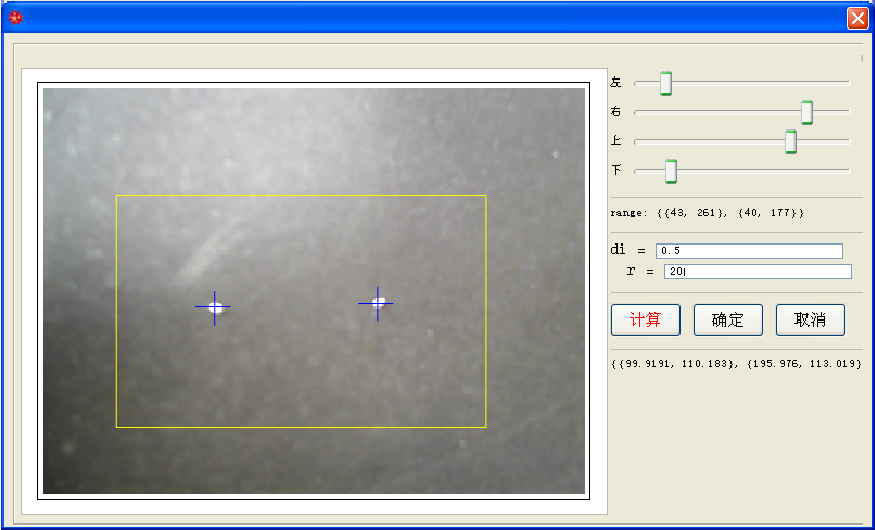
\includegraphics[width=100mm]{image/twospots-detect.pdf}
\caption{两个斑点的位置检测}\label{fig:twospots-detect}
\end{figure}


\subsection{薄膜厚度和平整度的自动化测量}

镀在基底上的薄膜的厚度一般是很微小的,薄膜厚度的变化程度,即平整度也是不容易测量的。该项目是利用激光
干涉法对薄膜的厚度和平整度进行测量,采用的是分振幅等倾干涉法,一束激光沿水平方向以45度角斜射到半透
半反镜上,激光光线会竖直向下分为两束平行光照射在基底上,基底沿水平方向放置,它会把两束光线竖直向上
原路反射回去,两束光线经过半透半反镜上方的凸透镜聚焦到接受光屏(焦平面)上发生干涉,当基底向一个方
向移动时,
其中一束激光会先遇到薄膜,由于薄膜厚度的存在,会使这束激光光程变短,进而使接收光屏上的干涉条纹发生
移动。记录下当这束激光完全照射在薄膜上时干涉条纹的移动数量,就可以计算出薄膜的厚度。薄膜平整度的测量
则是把两束激光都照射在薄膜上,当薄膜移动时,薄膜厚度的变化也会使两束激光的光程差改变,以致干涉条纹
发生移动,这个移动数量可以用于衡量薄膜的平整度。

图\;\ref{fig:baomohoudu} 是为该项目开发的程序系统的界面。该程序的核心内容就是对定点干涉条纹扫过数量
的自动计数。在程序界面的中间就是上述的干涉条纹移动数量自动计数模块。在最上边一排按钮的最左边是
``参数设置''按钮,用于向程序输入仪器相关参数和条纹计数程序所需的三个统计量参数\verb|imin|、
\verb|imax|和\verb|igap|。如前所述,在开始拍摄之前是不能进行条纹计数的,单击``开始拍摄''按钮,
就会把启动程序\verb|fringesDataGet[ ]|,其运行效果见图\;\ref{fig:fringes-count} ,该程序开始动态
刷新全局变量\verb|fringesData|。然后计数按钮被激活,``未能计数''变为``开始计数'',单击``开始计数''
按钮,就可以启动计数程序\verb|fringesCount[ ]|,开始即时跟踪检查全局变量\verb|fringesData|,自动
分析条纹的特征,对条纹的移动数量进行计数,计数结果会随时传递给全局变量\verb|counter|(计数器)和
\verb|total|(总条纹数)。计数结果会在拍摄图像下方以\verb|Dynamic[ ]|结构的形式在界面中输出。
程序界面下方的四个滑块分别用于调整图像中指定进行条纹计数的定点位置和设置扫描和采样数据量的大小。
由于薄膜平整度测量采用了多次扫描的方法,就是在待测平面上的不同位置进行多次测量,然后综合评定
薄膜平面的平整度,其中需要对多个条纹数量以一定的规则进行分组,在该程序中对条纹计数程序
\verb|fringesCount[ ]|做了一些改进,具体内容不再详述。在每一次更换扫描位置时,都应该单击一下
``记录''按钮,按钮中的数字表示记录的个数,也是扫描位置更换的次数。


\begin{figure}[htbp]
\centering
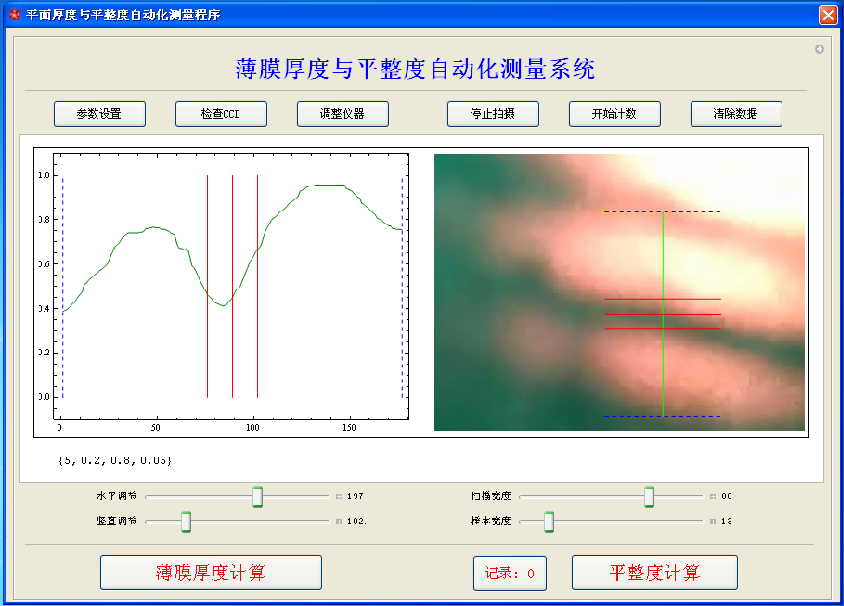
\includegraphics[width=115mm]{image/baomohoudu.pdf}
\caption{薄膜厚度和平整度自动化测量程序}\label{fig:baomohoudu}
\end{figure}



\section{结论}
本文详细地探讨了CCD图像中激光斑点位置的提取算法、扫过定点的激光干涉条纹数量的自动计数方法,并对
实际使用的整个软件系统所需要的程序模块的构建和整体系统的组建方法做了详细地论述和说明。实际的使用
和测试,证明了本文论述
的算法和程序的可靠性。这些算法和程序大大提高了利用激光进行微位移测量相关的仪器设备的工作效率,
节省了大量不必要的人力的耗费。在2011年和2012年两届山东省大学生
物理科技创新大赛中,这些算法和程序得到了充分的应用,开发了一系列应用软件系统,并取得了很好的成绩。


%% -------------------------------------------------------------------------------

%% ================================= 参考文献 =====================================


\bibliographystyle{GBT7714-2005N}\bibliography{bibdata}
\addcontentsline{toc}{section}{参考文献}

%% -------------------------------------------------------------------------------

%% =================================== 致谢 =======================================

\addcontentsline{toc}{section}{致谢}
\section*{致谢}

这篇论文中所涉及的算法和程序都是我在2011年和2012年两届山东省大学生物理科技创新大赛中由于
实际项目的需要而探索研发出来的,这要十分感谢带领和指导我们参加这项比赛的张志峰老师,是
张老师给了我们大量动手实践的机会。在程序设计之初,要感谢油涵真学姐给我提供的程序界面样图,
她参加比赛时所用的程序是请其他学院的老师编制的,这给了我打算自己研发相关程序软件的想法和
灵感。在这篇论文的最后一节所列举的四个参赛项目分别是由蔡亚丽、张广迪、马昆和许永娜发起的,
感谢他们研制的测量仪器,为这篇论文所述的算法和程序提供了测试和应用的平台。还要感谢张荣真、
孙永利以及其他所有和我一起参加过比赛的队友们在比赛和生活中各方面给我的很多关心和帮助。

谨以此文献给陪伴我大学四年的鲁东大学科技创新协会!
%% -------------------------------------------------------------------------------

%% =================================== 附录 =======================================
\newpage
\addcontentsline{toc}{section}{附录}
\section*{附录}
\appendix

\section{附录一:多斑点定位程序代码}
\subsection{函数:briPointHole[ ]}
\begin{verbatim}
briPointHole[imgdata_, hole_, dim_:{240,320}] := Module[{
    L, l, max = 0, tmp, x, y
    },
    {L, l} = dim;
    (*一个原则:输入和输出的坐标都是几何坐标*)
    (*几何坐标是指以图像左下角为坐标原点*)
    Do[
        If[!MemberQ[hole, {j, L - i + 1}], 
            tmp = 0.299 * imgdata[[i, j, 1]] + 0.587 * imgdata[[i, j, 2]] 
                  + 0.114 * imgdata[[i, j, 3]];
            If[tmp > max,
                max = tmp; x = j; y = L - i + 1;
            ]
        ],
        {i, 1, L}, {j, 1, l}
    ];
    {x, y}
];
\end{verbatim}

\subsection{函数:pointsDetect[ ]}
\begin{verbatim}
pointDetect[imgdata_, centerG_, maxR_, dim_:{240, 320}, di_:0.1] := Module[{
    L, l,
    tmp, max,
    center, tmpcen, point,
    totalPoints = { }, innerPoints = { }, outerPoints = { },
    m, n, x, y, hole = { }
    },
    {L, l} = dim;
    center = {L - centerG[[2]] + 1, centerG[[1]]};
    {m, n} = center;
    max = 0.299 * imgdata[[i, j, 1]] + 0.587 * imgdata[[i, j, 2]] 
          + 0.114 * imgdata[[i, j, 3]];
    outerPoints = totalPoints = {center}; (*初始化点集*)
    While[Length[outerPoints] > 0,
        innerPoints = outerPoints;
        outerPoints = { };
        Do[
            tmpcen = innerPoints[[i]];
            (*限制探测范围*)
            If[(Norm[tmpcen - center] < maxR) 
                && (2 < tmpcen[[1]] < L - 1) 
                && (2 < tmpcen[[2]] < l - 1),
                (*探测内层点上下左右像素点是否满足亮度条件*)
                Do[
                    {m, n} = point;
                    tmp = 0.229 * imgdata[[m, n, 1]] 
                          + 0.587 * imgdata[[m, n, 2]]
                          + 0.114 * imgdata[[m, n, 3]];
                    If[(max - di <= tmp <= max) 
                        && (!MemberQ[totalPoints, point]),
                        AppendTo[outerPoints, point]; 
                        AppendTo[totalPoints, point];
                    ],
                    {point, {
                        {tmpcen[[1]], tmpcen[[2]] - 1}, (*左*)
                        {tmpcen[[1]], tmpcen[[2]] + 1}, (*右*)
                        {tmpcen[[1]] - 1, tmpcen[[2]]}, (*上*)
                        {tmpcen[[1]] + 1, tmpcen[[2]]}  (*下*)
                    } }
                ] (* Do *)
            ], (* If *)
            {i, 1, Length[innerPoints]}
        ] (* Do *)
    ]; (* While *)
    {m, n} = N@Mean[totalPoints];
    {x, y} = {n, L - m + 1}; (*把像素点坐标转化为几何坐标*)
    Do[
        AppendTo[hole, {totalPoints[[i,2]], L - totalPoints[[i, 1]] + 1}],
        {i, 1, Length[totalPoints]}
    ];
    {{x, y}, hole}
];
\end{verbatim}

\subsection{函数:multiSpots[ ]}
\begin{verbatim}
multiSpots[imgdata_, n_, maxR_, dim_:{240, 320},di_:0.1] := Module[{
    briPoint, briPoints = { }, hole, holes = { }, centerG
    },
    Do[
        centerG = briPointHole[imgdata, Flatten[holes,1],dim];
        {briPoint, hole} = pointsDetect[imgdata, centerG, maxR, dim, di];
        AppendTo[briPoints, briPoint];
        AppendTo[holes, hole],
        {n}
    ];
    {briPoints, holes}
]
\end{verbatim}

\section{附录二:函数briPointExpand[ ]的编译版本}
\begin{verbatim}
briPointExpandC = Compile[{
 {imgdata, _Real, 3},
 {maxR, _Integer},
 {dim, _Integer, 1},
 {di, _Real}
 },
 Module[{
    L = 1, l = 1,
    tmp = 0.0, max = 0.0,
    center = {0, 0}, tmpcen = {0, 0}, point = {0, 0},
    totalPoints = {{0, 0}}, innerPoints = {{0, 0}}, outerPoints = {{0, 0}},
    m = 1, n = 1, rsm = 0.0, rsn = 0.0, y = 0.0, len = 0, cc = {0, 0}
    },
    {L, l} = dim;
    (*先用擂台算法找出最亮像素点的位置和亮度值*)
    Do[ 
        tmp = 0.299 * imgdata[[i,j,1]] + 0.587 * imgdata[[i,j,2]]
              +0.114 * imgdata[[i,j,3]];
        If[tmp > max,
            max = tmp; center = {i, j};
        ],
        {i, 1, L}, {j, 1, l}
    ];
    AppendTo[outerPoints,center];
    totalPoints = {center};         (*初始化点集*)
    While[Length[outerPoints] > 1,
        innerPoints = Drop[outerPoints, 1];
        outerPoints = {{0, 0}};
        Do[
            tmpcen = innerPoints[[i]];
            (*限制探测范围*)
            cc = tmpcen - center;
            If[(cc[[1]]^2 + cc[[2]]^2 < maxR^2) 
                && (2 < tmpcen[[1]] < L - 1) 
                && (2 < tmpcen[[2]] < l - 1),
                (*探测内层点上下左右像素点是否满足亮度条件*)
                Do[
                    {m, n} = point;
                    tmp = 0.229 * imgdata[[m, n, 1]] 
                          + 0.587 * imgdata[[m, n, 2]]
                          + 0.114 * imgdata[[m, n, 3]];
                    If[(max - di <= tmp <= max) 
                        && (!MemberQ[totalPoints, point]),
                        AppendTo[outerPoints, point]; 
                        AppendTo[totalPoints, point];
                    ],
                    {point, {
                        {tmpcen[[1]], tmpcen[[2]] - 1}, (*左*)
                        {tmpcen[[1]], tmpcen[[2]] + 1}, (*右*)
                        {tmpcen[[1]] - 1, tmpcen[[2]]}, (*上*)
                        {tmpcen[[1]] + 1, tmpcen[[2]]}  (*下*)
                    } }
                ] (* Do *)
            ], (* If *)
            {i, 1, Length[innerPoints]}
        ] (* Do *)
    ]; (* While *)
    len = Length[totalPoints];
    Do[
        rsm += totalPoints[[i, 1]]; rsn += totalPoints[[i,2]],
        {i, 1, len}
    ];
    {x, y} = {rsn/len, L - rsm/len + 1}; 
    {x, y}
]
\end{verbatim}

\section{附录三:程序模块设计相关的程序代码}

\subsection{函数: processCCD[ ]}
\begin{verbatim}
processCCD[curimg_, originalPosition_, start_:False, maxR_:10,
  dim_:{240, 320}, di_:0.1, size_:300] := Module[{
    L, l,
    result (*可视化结果*)
    (* currentPosition 为全局变量,记录提取到的激光斑点的即时位置 *)
    (* currentDistance 为全局变量,记录当前激光斑点位移的像素距离 *)
    },
    {L, l} = dim;
    If[start,
        (*开始监控*)
        (*计算并更新当前激光斑点的位置坐标*)
        currentPosition = briPointExpandC[ImageData[curimg],maxR,dim,di];
        currentDistance = currentPosition - originalPosition;
        (*可视化激光斑点的初始位置和即时位置*)
        result = Show[curimg,
            Graphics[{
                Blue,  (*标明激光斑点的即时位置*)
                Line[{{0,currentPosition[[2]]},{l,currentPosition[[2]]}}],
                Line[{{currentPosition[[1]],0},{currentPosition[[1]],L}}],
                Dashed, Red,  (*标明激光斑点的初始位置*)
                Line[{{0,originalPosition[[2]]},{l,originalPosition[[2]]}}],
                Line[{{originalPosition[[1]],0},{originalPosition[[1]],L}}],
                Yellow, Arrow[{originalPosition, currentPosition}]
            }],
            ImageSize -> size
        ],
        (*还未开始监控*)
        result = Show[curimg,
            Graphics[{
                Dashed, Red,   (*标明激光斑点的初始位置*)
                Line[{{0,originalPosition[[2]]},{l,originalPosition[[2]]}}],
                Line[{{originalPosition[[1]],0},{originalPosition[[1]],L}}]
            }],
            ImageSize -> size
        ]
    ];
    (*输出结果*)
    Column[{
        Framed[result],
        Row[{
            StringForm["P0:(`1`,`2`)", 
                NumberForm[originalPosition[[1]], {3, 0}],
                NumberForm[originalPosition[[2]], {3, 0}] ],
            StringForm["P1:(`1`,`2`)", 
                NumberForm[currentPosition[[1]], {3, 0}],
                NumberForm[currentPosition[[2]], {3, 0}] ],
            StringForm["P1-P0 = `1`", 
                NumberForm[N@Norm[currentDistance], {3, 0}] ]
            }, 
            Spacer[5]
        ]
    }]
]
\end{verbatim}

\subsection{函数:getProportion[ ]}

\begin{verbatim}
getProportion[] := CreateWindow[DialogNotebook[
  DynamicModule[{
   tmpimg, (*临时储存CCD图像*)
   points, (*手动取得的两个点坐标*)
   actualDistance, (*两点的实际距离,以厘米为单位*)
   tmpProportion  (*临时储存算出的比例系数*)
   (* proportion 为全局变量,用于向其他模块传递测得的比例系数*)
   },
   Manipulate[
    Framed@Dynamic[Show[tmpimg, ImageSize -> 400]],
    Item[
        Row[{Null, #},Spacer[60]]&@Column[{
            Button["拍摄", 
                tmpimg := CurrentImage[], 
                ImageSize -> {150, 26}
            ],
            Button["拍照",
                tmpimg = CurrentImage[],
                ImageSize -> {150, 26}
            ]
        }], 
        ControlPlacement -> Right ],
    Delimiter,
    Item[Grid[{
        {"Points: ", InputField[Dynamic[points]],Null},
        {"acDist: ", InputField[Dynamic[actualDistance]]," cm"},
        },
        Alignment -> {{Right, Center, Left}, {Right, Center, Left}},
        Frame -> {None, {{True}}},
        FrameStyle -> GrayLevel[0.6],
        Spacings -> {0, 2} ], 
      ControlPlacement -> Right ],
    Delimiter,
    Item[Column[{
        Button[Style["计算", {Red, 15}],
            (If[actualDistance != 0,
                tmpProportion = 
                      Norm[points[[1]] - points[[2]]]/actualDistance;
            ]),
            ImageSize -> {150, 30} ],
        Row[{
            "prop = ",
            InputField[Dynamic[tmpProportion], FieldSize->18],
            " px/cm" }],
        Button["确定", 
            proportion = tmpProportion; DialogReturn[],
            ImageSize->{150, 30}]
        }, 
        Center, Spacings -> 2, Frame -> All, 
        FrameStyle -> GrayLevel[0.6] ],
      ControlPlacement -> Right
    ],
    AppearanceElements -> None,
    Initialization :> (
        tmpimg := CurrentImage[]; points = {{0, 0}, {0, 0}};
        actualDistance = 0; tmpProportion = proportion )
   ]
  ], WindowTitle -> "比例系数测量", WindowSize -> All
]]
\end{verbatim}

\newpage
\section{附录四:历年获奖情况}
\noindent 2011年-山东省第三届大学生物理科技创新大赛:
\begin{itemize}
\item 计算机全真模拟下的对碰撞打靶能量损失的进一步研究 \hfill \emph{一等奖}
\item 垂直摆倾斜仪数据采集与分析系统 \hfill \emph{特等奖}
\item 旋转液体物理特性研究实验改进的数据处理程序 \hfill \emph{一等奖}
\item 折射率自动化测量程序 \hfill \emph{一等奖}
\item 薄膜厚度与平整度自动化测量系统 \hfill \emph{一等奖}
\item 微小角度实时测量程序 \hfill \emph{二等奖}
\item 地磁场水平分量自动化测量程序 \hfill \emph{二等奖}
\item 粘滞系数计算程序 \hfill \emph{二等奖}
\end{itemize}

\noindent 2012年-山东省第四届大学生物理科技创新大赛:
\begin{itemize}
\item 液体表面张力系数自动化测量系统 \hfill \emph{特等奖}
\item 实时地倾斜及地震监测与预警系统 \hfill \emph{二等奖}
\item 劈尖干涉法液体折射率自动化测量程序 \hfill \emph{一等奖}
\item 大学物理实验导学系统 \hfill \emph{一等奖}
\end{itemize}

\noindent 2012年-数学建模
\begin{itemize}
\item 美国大学生数学建模竞赛(MCM) \hfill \emph{Honorable Mention(二等奖)}
\item 中国大学生数学建模竞赛(CUMCM) \hfill \emph{成功参赛}
\end{itemize}














\end{document}

